\documentclass[12pt,a4paper]{scrartcl}

%XeTeX блок:
\usepackage{xunicode}
\usepackage{xltxtra}

\setsansfont{CMU Sans Serif}
\setmainfont{CMU Serif}

\defaultfontfeatures{Scale=MatchLowercase,Mapping=tex-text}
% -- END --

%LaTeX блок:
%\usepackage[utf8]{inputenc}
% -- END --
\usepackage[russian]{babel}
\usepackage[OT1]{fontenc}



\usepackage{amsmath}
\usepackage{amsfonts}
\usepackage{amssymb}
\usepackage{graphicx}
\usepackage{hyperref}

\author{Алексей Лобанов}
\title{Анализ тем на TED}

%\date{ Today}
\makeindex
\begin{document}
\maketitle
\tableofcontents

\section{Введение}
В данном исследование рассмотрим некоторые особенности категоризации роликов на TED, найдём наиболее интересные пользователям темы и ролики

\section{Порядок работы}
С помощью scrapy был написан парсер, который за несколько часов собрал информацию по всем роликам. Я получал следующие данные:
\begin{enumerate}
\item Название ролика.
\item Список тегов.
\item Численное значение (не в виде процентов, как на сайте) каждой из зрительских оценок.
\item Количество просмотров.
\end{enumerate}

Как источник тем для видео возьмём теги. В самом деле, если эти видео уже категоризованы, то лучше этим воспользоваться
Всего 2133 видео и 357 тегов.
\subsection{Обзор тегов и их очистка}
Построим зависимость числа тегов, которые встретились хотя бы $n$ раз от $n$. Можно предположить, что будет гипербола. График~\ref{tags_from_val} это подтверждает.
\begin{figure}[hbp]
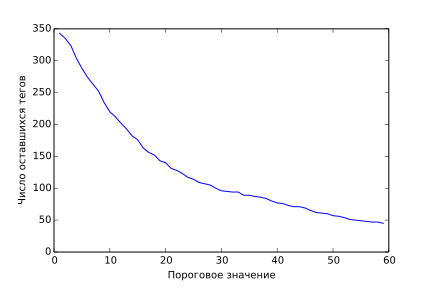
\includegraphics{tags_from_val.pdf}
\caption{Зависимость числа тегов от порогового значения}
\label{tags_from_val}
\end{figure}

Давайте более детально проанализируем теги. Их достаточно мало, чтобы это можно было сделать вручную. Заметим, что среди них встречаются такие, которые не относятся к тематике ролика, например, \emph{TED Conference} встретился 709 раз (33\% от всех видео). По этим причинам, давайте удалим следующие теги: TED Conference, TEDx, happiness (слишком общее), TED Brain Trust, data (слишком общее), TED Prize, TED-Ed, TEDYouth, choice (слишком общее), materials (слишком общее), MacArthur grant, TED Books, TEDMED.

Заметим также, что существует значительное число тегов, которые встречаются слишком редко, чтобы можно было считать их значимыми. В качестве порога было выбрано число три. Если тег встречается реже, чем в \emph{трёх} роликах, то мы его удаляем. Таким образом, будут удалены следующие теги: Moon, code, mobility, cloud, programming, capitalism, pandemic, urban, mining, TEDMED (этот тег редко встречается и не является темой), nuclear weapons, microsoft, Brand, testing, skateboarding, origami, vulnerability, evil, South America, glacier, cyborg, painting.

После удаления этих тегов, их осталось 323.
\subsection{Объединение тегов}
Рассмотрим две функции:
\begin{itemize}
\item Расстояние Жаккара:
$$\rho_J\left( A, B \right) = 1 - \frac{\left|A \cup B\right|}{\left| A \cap B \right|}$$
Это классическое расстояние поможет определить максимально близкие теги.

\item Мера Шимкевича-Симпсона:
$$\rho'\left( A, B \right) = 1 - \max \left( \frac{\left|A \cap B\right|}{|A|} , \frac{\left|A \cap B\right|}{|B|} \right)$$
Такая функция расстояния удобна для определения того, что какое-то множество \emph{почти} включает другое
\end{itemize}

Мне кажется разумным выдвинуть следующие гипотезы по тегам:
\begin{enumerate}
\item Есть очень много \emph{похожих} тегов, которые можно будет объединить.
\item Некоторые теги могут содержать другие почти полностью, то есть может существовать некая  иерархия.
\end{enumerate}
Начать проверку можно с первой. В таком случае будет удобно рассматривать расстояние Жаккара. Тогда есть лишь одна пара тегов, для которой данное расстояние меньше $0.5$, это пара \textit{meditation} и \textit{mindfulness}. Каждому из этих тегов принадлежат 4 одинаковых видео. Таким образом, можно удалить один из них, например, mindfulness. Это гипотеза неверна.

Рассмотрим вторую гипотезу. Есть 29 пар тегов, для которых один из них полностью содержит другой, например global issues и population. Построим граф~\ref{tags_graph}, показывающей иерархию тегов (рассматриваются с расстоянием Жаккара не более $0.15$).
\begin{figure}[hbp]
\includegraphics{tags_graph.pdf}
\caption{Иерархия тегов}
\label{tags_graph}
\end{figure}
Видно, что получилось несколько больших групп с центрами в тегах technology, science, music. Таким образом, можно считать эту гипотезу верной.

\subsection{Анализ просмотров}
Среднее число просмотров 1433164, медиана 973111. Построим распределение числа просмотров ~\ref{views}.
\begin{figure}[hbp]
\includegraphics{views.pdf}
\caption{Распределение числа просмотров}
\label{views}
\end{figure}
Самые популярные ролики:
\begin{enumerate}
\item Do schools kill creativity? и 37124197 просмотров
\item Your body language shapes who you are и 31154001 просмотров
\item How great leaders inspire action и 25449477 просмотров
\item The power of vulnerability и 23416955 просмотров
\item My stroke of insight и 18430876 просмотров
\item 10 things you didn't know about orgasm и 18195966 просмотров
\item Why we do what we do и 16146117 просмотров
\item The puzzle of motivation и 15014711 просмотров
\item The thrilling potential of SixthSense technology и 14464629 просмотров
\item Looks aren't everything. Believe me, I'm a model. и 13116493 просмотров
\end{enumerate}
Видно, что разница между первым и десятым роликами по числу просмотров "--- $2.8$ раза.

Самые популярные темы, по среднему числу просмотров:
\begin{enumerate}
\item succ и 6590998 просмотров
\item body language и 6118118 просмотров
\item Buddhism и 4036186 просмотров
\item goal-setting и 3788322 просмотров
\item dance и 3635241 просмотров
\item psychology и 3499243 просмотров
\item magic и 3473116 просмотров
\item motivation и 3473039 просмотров
\item fear и 3352476 просмотров
\item self и 3344291 просмотров
\end{enumerate}

Видно, что разница между первым и десятым роликами по числу просмотров "--- $2$ раза.
\subsection{Анализ пользовательских рейтингов}
Пользователь может оценить каждый из роликов одним из следующих рейтингов (можно выбрать до трёх, если выбран один, то он учитывается трижды):
\begin{enumerate}
\item beautiful
\item inspiring
\item informative
\item fascinating
\item OK
\item persuasive
\item jaw-dropping
\item ingenious
\item courageous
\item confusing
\item obnoxious
\item longwinded
\end{enumerate}
Отдельный анализ по всем этим рейтингам малополезен, так как такие, как OK не несут практически никакой информации. Тем не менее, некоторые из них вполне достойны некоторого анализа.

Будем ранжировать ролики по параметру $R / V$, где $R$ и $V$ это количество данных рейтингов и количество просмотров соответственно. Для упорядочивания рейтингов воспользуемся параметром $\left( \sum_{R_i \in R} R_i \right) / \left( \sum_{V_i \in V} V_i \right)$, где $R$ и $V$ это множества данных рейтингов и просмотров роликов данного тега соответственно.
\subsubsection{Анализ по рейтингу beautiful}
Начнём с 5 роликов с самым большим параметром: 
\begin{enumerate}
\item Kounandi, у которого 70851 просмотров
\item How many lives can you live?, у которого 514237 просмотров
\item The secret life of plankton, у которого 182096 просмотров
\item M'Bifo, у которого 264956 просмотров
\item A message to gay teens: It gets better, у которого 264170 просмотров
\end{enumerate}
Далее, 5 тегов с самым большим значением данного параметра:
\begin{enumerate}
\item Foreign Policy
\item conducting
\item guitar
\item violin
\item cello
\end{enumerate}
\subsubsection{Анализ по рейтингу inspiring}
Начнём с 5 роликов с самым большим параметром: 
\begin{enumerate}
\item Transplant cells, not organs, у которого 591904 просмотров
\item A message to gay teens: It gets better, у которого 264170 просмотров
\item When a reporter becomes the story, у которого 118258 просмотров
\item Which country does the most good for the world?, у которого 2194074 просмотров
\item Why we all need to practice emotional first aid, у которого 3105779 просмотров
\end{enumerate}
Далее, 5 тегов с самым большим значением данного параметра:
\begin{enumerate}
\item Foreign Policy
\item chautauqua
\item Latin America
\item Buddhism
\item death
\end{enumerate}
\subsubsection{Анализ по рейтингу informative}
Начнём с 5 роликов с самым большим параметром: 
\begin{enumerate}
\item The early birdwatchers, у которого 108989 просмотров
\item Just how small is an atom?, у которого 349159 просмотров
\item What happens when an NGO admits failure, у которого 202608 просмотров
\item Inventing is the easy part. Marketing takes work, у которого 179460 просмотров
\item The sea we've hardly seen, у которого 135665 просмотров
\end{enumerate}
Далее, 5 тегов с самым большим значением данного параметра:
\begin{enumerate}
\item oil
\item privacy
\item human origins
\item wind energy
\item presentation
\end{enumerate}
\subsubsection{Анализ по рейтингу obnoxious}
Это пример рейтинга, который, как мне кажется, следует считать негативным. Начнём с 5 роликов с самым большим параметром: 
\begin{enumerate}
\item 17 words of architectural inspiration, у которого 680410 просмотров
\item I believe we evolved from aquatic apes, у которого 987158 просмотров
\item Protecting the brain against concussion, у которого 394909 просмотров
\item Put the financial aid in the bag, у которого 164513 просмотров
\item Gotta share!, у которого 349869 просмотров
\end{enumerate}
Далее, 5 тегов с самым большим значением данного параметра:
\begin{enumerate}
\item apes
\item Christianity
\item oil
\item atheism
\item God
\end{enumerate}
Кажется весьма логичным, что такие спорные категории, как Christianity, atheism и God попали в этот список.
\subsubsection{Анализ активности}
Давайте введём параметр активность. Для ролика определим его так: $\sum_{R_i \in R} / V$, где где $R$ и $V$ это множество с рейтингами и количество просмотров данного ролика соответственно. Тогда, по аналогии, на тег это можно обобщить как:
$$ \left( \sum_{R^k \in R} \sum_{R_i \in R^k} R_i \right) / \left( \sum_{V_i \in V} V_i \right) $$
Здесь $R$ это множество множеств рейтингов каждого из роликов, а $V$ множество с просмотрами каждого из роликов.

Начнём с 5 роликов с с самым большим параметром: 
\begin{enumerate}
\item A message to gay teens: It gets better, у которого 264170 просмотров
\item Transplant cells, not organs, у которого 591904 просмотров
\item The case for same-sex marriage, у которого 284271 просмотров
\item "Kounandi", у которого 70851 просмотров
\item What happens when an NGO admits failure, у которого 202608 просмотров
\end{enumerate}
Далее, 5 тегов с самым большим значением данного параметра:
\begin{enumerate}
\item oil
\item Foreign Policy
\item illness
\item apes
\item consciousness
\end{enumerate}
Видно, что у этих роликов достаточно мало просмотров. Давайте посмотрим ~\ref{running_mean} на значение этого параметра, в зависимости от числа просмотров ролика. Легко заметить, что график достаточно ровный, за исключением роликов с небольшим числом просмотров. Таким образом, можно сделать вывод, что эта характеристика малоинформативна.
\begin{figure}[hbp]
\includegraphics{running_mean.pdf}
\caption{Распределение значения параметра, после применения скользящего среднего}
\label{running_mean}
\end{figure}
\section{Инструменты}
При исследовании были использованы следующие инструменты:
\begin{description}
\item[Python] "--- основной язык программирования при исследовании.
\item[Scrapy] "--- библиотека для написания парсера.
\item[PyLab] "--- создание графиков.
\item[Numpy] "--- некоторые статистические функции.
\item[Ipython] "--- утилита для более удобного исследования данных.
\item[Graph\_tool] "--- библиотека для работы с графами.
\item[XeTeX] "--- создания отчёта.
\end{description}
\section{Выводы}

\subsection{Получение данных}
Несмотря на то, что TED достаточно открыто делится со всем миром своими выводами, API был закрыт. Мне кажется, что если бы был API, то удалось бы больше усилий приложить непосредственно к исследованию.

Слишком частые запросы завершались сервером с ошибкой 329.
\subsection{Теги}
Теги являются самыми очевидными индикаторами темы выступления. Гипотеза о том, что их можно было объединять с тем, чтобы сократить их количество не оправдалась, хотя предполагалось, что это выполняется из-за большого их числа.
\subsection{Работа с субтитрами}
Как мне кажется, работа с субтитрами затруднена, применительно к данному исследованию. В самом деле, получать темы бессмысленно, так как они уже есть в тегах, получать же более специфические темы тоже бессмысленно, так анализ таких редких тем будет малополезен.

Единственное применение, которое я смог найти "--- анализ эмоциональной составляющей доклада. Но для этого нужна размеченная база со словами, и мне кажется, что это не совсем соотносится с темой исследования.
\subsection{Направления для дальнейшей работы}
\begin{enumerate}
\item Анализ эмоциональности докладов, по субтитрам
\item Добавление к данным авторов (есть авторы, которые выступали более раза). Поиск наиболее успешных авторов.
\item Добавление к данным длительности роликов. Поиск возможных зависимостей между длительностью и какими-либо рейтингами (например, между длительностью и рейтингом longwinded)
\end{enumerate}
\end{document}